%CLASSE DOCUMENTO - LINGUA E DIMENSIONE FONT
\documentclass[corpo=13pt,numerazioneromana]{toptesi}

%%%%%%%%%%%%%%%%%%%%%%%%%%%%%%%%%%%%%%%%%%%%%%%%%%%%%%%%%%%%%%%

% INCLUSIONE PACCHETTI
\usepackage[classica]{topfront}
\usepackage[utf8]{inputenc} %utf8
\usepackage[italian]{babel}
\usepackage[T1]{fontenc}
\usepackage{blindtext}
\usepackage{graphicx,wrapfig}
\usepackage{booktabs}
\usepackage{lmodern}
\usepackage{varioref}
\usepackage{url}
\usepackage{array}
\usepackage{paralist}{\obeyspaces\global\let =\space}
\usepackage{verbatim}
\usepackage{subfig}
\usepackage{tabularx}
\usepackage{amsmath}
\usepackage{amsfonts}
\usepackage{float}
\usepackage{amssymb}
\usepackage{multicol}
\usepackage{multirow}
\usepackage{listings}
\usepackage[pass]{geometry}
\usepackage[figuresright]{rotating}
\usepackage{algorithm}
\usepackage{algorithmic}
\usepackage{amsmath}
\usepackage[babel]{csquotes}
\usepackage{hyperref}
\usepackage[backend=biber,bibencoding=ascii]{biblatex}


%%%%%%%%%%%%%%%%%%%%%%%%%%%%%%%%%%%%%%%%%%%%%%%%%%%%%%%%%%%%%%%

% CONFIGURAZIONE LINK E RIFERIMENTI
\hypersetup{%
    pdfpagemode={UseOutlines},
    bookmarksopen,
    pdfstartview={FitH},
    colorlinks,
    linkcolor={black}, %COLORE DEI RIFERIMENTI AL TESTO
    citecolor={blue}, %COLORE DEI RIFERIMENTI ALLE CITAZIONI
    urlcolor={blue} %COLORI DEGLI URL
}

%%%%%%%%%%%%%%%%%%%%%%%%%%%%%%%%%%%%%%%%%%%%%%%%%%%%%%%%%%%%%%%

% CONFIGURAZIONE LISTATI/CODICE - CANCELLARE SE NON NECESSARIO
% PYTHON - BIANCO E NERO
\lstset{%
	captionpos=b,
	language=Python,
	basicstyle =\small\ttfamily,
	keywordstyle=\color{black}\bfseries,
	breaklines=true,
	breakatwhitespace=true,
	frame=lines,
	numbers=left,
	numberstyle=\footnotesize,
}

%%%%%%%%%%%%%%%%%%%%%%%%%%%%%%%%%%%%%%%%%%%%%%%%%%%%%%%%%%%%%%%

% FRENCHSPACING VA _SEMPRE_ ABILITATO PER DOCUMENTI IN ITALIANO
\frenchspacing

%%%%%%%%%%%%%%%%%%%%%%%%%%%%%%%%%%%%%%%%%%%%%%%%%%%%%%%%%%%%%%%

%DEFINIZIONE SEZIONI IN NUMERAZIONE ROMANA
%ELENCO DEI LISTATI/CODICI
\makeatletter
\newcommand\listofcodes{%
 \iffrontmatter\else\frontmattertrue\fi
 \if@openright\cleardoublepage\else\clearpage\fi
 % change the meaning of \chapter in a group
 \begingroup\def\chapter##1{\@schapter}
 \phantomsection % for the hyperlink
 \addcontentsline{toc}{chapter}{Elenco dei listati}
 \lstlistoflistings
 \endgroup
} 
\makeatother

\addto\captionsitalian{%
  \renewcommand{\lstlistlistingname}{Elenco dei listati}%
  \renewcommand{\lstlistingname}{Listato}%
}

%%%%%%%%%%%%%%%%%%%%%%%%%%%%%%%%%%%%%%%%%%%%%%%%%%%%%%%%%%%%%%%

% INFORMAZIONI PDF - PERSONALIZZARE
\pdfinfo{%
  /Title    (Cubo cloud computing web content management system)
  /Author   (Luca Mantovani)
  /Subject  (Tesi di laurea sull'attività di tirocinio)
  /Keywords (Cubo Laurea Tesi Ingegneria)
}

%%%%%%%%%%%%%%%%%%%%%%%%%%%%%%%%%%%%%%%%%%%%%%%%%%%%%%%%%%%%%%%

% LISTA DEI CAPITOLI DA INCLUDERE - PERSONALIZZARE
\includeonly{%
chap_1,%
chap_2,%
chap_3,%
chap_4,%
chap_5,%
}

% FILE DI BIBLIOGRAFIA
\addbibresource{bibliography.bib}

%%%%%%%%%%%%%%%%%%%%%%%%%%%%%%%%%%%%%%%%%%%%%%%%%%%%%%%%%%%%%%%

% INIZIO DOCUMENTO
\begin{document}

%%%%%%%%%%%%%%%%%%%%%%%%%%%%%%%%%%%%%%%%%%%%%%%%%%%%%%%%%%%%%%%

% FRONTESPIZIO - PERSONALIZZARE
% ELIMINATE LE VOCI CHE NON VI SERVONO

% UNIVERSITA - NOME
\ateneo{Università degli studi di Modena e Reggio Emilia}

% FACOLTA - DICITURA - CANCELLARE O DECOMMENTARE
\FacoltaDi{Dipartimento di Ingegneria "Enzo Ferrari"}
% FACOLTA - NOME
%\facolta{Ingegneria Informatica}

% CORSO DI LAUREA - DICITURA (MANTENERE LO SPAZIO) - CANCELLARE O DECOMMENTARE
\CorsoDiLaureaIn{Corso di Laurea in}
% CORSO DI LAUREA - NOME
\corsodilaurea{Ingegneria Informatica}

% TIPOLOGIA TESI
\TesiDiLaurea{Tesi di Laurea}

% TITOLO
\titolo{CUBO CLOUD COMPUTING WEB CONTENT MANAGEMENT SYSTEM}

% SOTTOTITOLO
\sottotitolo{Implementazione di un sistema per la gestione dei contenuti \break distribuito su infrastrutture cloud}

% RELATORE - PROF. NOME E COGNOME
\relatore{Claudia Canali}

% TUTORE AZIENDALE - TITOLO NOME E COGNOME
\tutoreaziendale{\break}
% TUTORE AZIENDALE - DICITURA//AZIENDA
\NomeTutoreAziendale{\break}

% CANDIDATO - DICITURA (MANTENERE I DUE PUNTI) - CANCELLARE O DECOMMENTARE
\CandidateName{Candidate:}

% CANDIDATO - NOME E COGNOME
\candidato{Luca Mantovani}

% DATA - MESE ANNO
\sedutadilaurea{Anno Accademico 2020/2021}

\frontespizio

%%%%%%%%%%%%%%%%%%%%%%%%%%%%%%%%%%%%%%%%%%%%%%%%%%%%%%%%%%%%%%%

%INTERLINEA - DEFAULT 1 - NON ESAGERATE, NON SUPERATE MAI 1.3 ;)
\interlinea{1.35}

%%%%%%%%%%%%%%%%%%%%%%%%%%%%%%%%%%%%%%%%%%%%%%%%%%%%%%%%%%%%%%%

%RINGRAZIAMENTI
\ringraziamenti
Prima di procedere con la trattazione, vorrei dedicare qualche riga a tutti coloro che mi sono stati vicini in questo percorso di crescita personale.
Innanzitutto, ringrazio il mio relatore, l'ing. Claudia Canali, sempre pronta a darmi le giuste indicazioni in ogni fase della realizzazione dell’elaborato. Ringrazio infinitamente i miei genitori senza i quali non sarei mai potuto arrivare fin qua. Grazie per avermi sempre sostenuto in ogni mia decisione e per esserci sempre stati nei momenti più difficili, siete la mia più grande ispirazione. Ringrazio la Dott.ssa Serena Zuliani per la professionalità e l'umanità dimostratemi in un momento particolare della mia vita, le sarò per sempre riconoscente. Ringrazio il Dott. Francesco Lotti per la sensibilità e la disponibilità con le quali ha prontamente deciso di prendermi in carico nel proseguo dei miei giorni. Ringrazio i miei amici, i miei compagni universitari e tutte le persone con le quali ho avuto modo di condividere emozioni, pensieri, parole e insicurezze, ve ne sarò per sempre grato. Infine, volevo ringraziare me stesso per il raggiungimento di questo grande traguardo e per aver portato al termine questo percorso con grande determinazione.



% INDICE GENERALE
\tableofcontents

% INDICE DELLE FIGURE
\listoffigures

%INDICE DEL CODICE
%\listofcodes

%%%%%%%%%%%%%%%%%%%%%%%%%%%%%%%%%%%%%%%%%%%%%%%%%%%%%%%%%%%%%%%

\mainmatter

% INCLUSIONE FILE CAPITOLI - PERSONALIZZARE - TENERE COERENTE CON LISTA IN ALTO
\chapter{Introduzione}
\label{chap:Introduction}

Internet ha completamente rivoluzionato la quotidianità, lo stile di vita e il modo di farsi conoscere. Gran parte della popolazione trascorre la maggior parte del suo tempo online, alla ricerca di informazioni e contenuti appaganti che possano soddisfare determinate esigenze. Il livello d'interazione con i siti web risulta elevatissimo e l'esperienza maturata durante il tirocinio mi ha permesso di addentrarmi all'interno di questo ambiente e poterne apprendere al meglio il suo funzionamento e la sua importanza.
L'attività è stata svolta presso l'azienda mantovana Studio Indaco, specializzata in pianificazione strategica per il web, realizzazione siti internet, campagne di web marketing e fotografia. Durante la pratica ho avuto modo di poter interagire con Cubo CMS (il sistema per la gestione dei contenuti alla base della realizzazione dei siti da parte della società in questione) e studiare l'infrastruttura architettata per poter erogare e gestire al meglio i servizi messi a disposizione.
Il principale obiettivo del tirocinio è stato quello di approfondire la conoscenza dei linguaggi di programmazione applicati al web tramite l'implementazione del sistema per la gestione dei contenuti nell'ottica della produzione di diversi siti su specifiche richieste dei clienti. \hfill \break \break
Il documento mette in relazione tutti gli aspetti del CMS utilizzato in fase di progettazione e si struttura nel seguente modo: il capitolo 2 presenta un excursus per quanto ne riguarda la storia e l'evoluzione che ha avuto questo tipo di strumento.
Il capitolo 3 analizza la struttura ed il modo secondo il quale è stato sviluppato e implementato il sistema. Il capitolo 4 descrive le infrastrutture e le soluzioni messa in pratica per la distribuzione del servizio. Il capitolo 5 riassume l'operato e conclude il documento.
\chapter{CMS: evoluzione e ruolo attuale}
\label{chap:CMSEvoluzioneRuolo}

%%%%%%%%%%%%%%%%%%%%%%%%%%%%%%%%%%%%%%%%%

Il CMS (content management system) è uno software applicativo lato server utilizzato per il coordinamento e la supervisione dei contenuti presenti in un determinato sito web. L'obiettivo è semplificare la gestione di tutti i vari elementi d'interesse indipendentemente dalle reali competenze tecniche di programmazione dell'utente incaricato per la gestione.\hfill \break


\section{Cenni storici, nascita e sviluppo}
I sistemi per la gestione dei contenuti nascono negli Stati Uniti ed inizialmente furono sviluppati ad uso privato per ovviare alla problematica amministrativa del gran quantitativo di pubblicazioni prodotte all'epoca.
Nel 1995 FileNet, un'azienda con sede in Costa Mesa (California), sviluppò un software che ad oggi può essere considerato il primo e vero content management system, strutturato secondo una suite di programmi per poter gestire i documenti in tutte le sue componentistiche (ovvero dal punto di vista del workflow, della parte grafica e di quella testuale). In maniera trasversale, nello stesso anno venne fondata la Vignette Corporation, un'azienda con sede ad Austin (Texas). 
La compagnia nacque dall'intento di andare a sviluppare uno strumento che permettesse una personalizzazione ed un'accessibilità più ampia all'interno del web development e nel 1996 venne pubblicato StoryBuilder, un sistema flessibile che permetteva la gestione dei contenuti su larga scala.
Durante il deployment, l'azienda texana strinse una collaborazione con CNET (abbreviazione di Computer Network), un sito web americano specializzato nella pubblicazione di articoli a tema tecnico-informatico, che nel contempo si mobilitò per sviluppare il proprio sistema di gestione dei contenuti, in seguito denominato PRISM, che introdusse l'utilizzo del database per la gestione interna dei dati. 
La svolta, in termini concettuali, avvenne nel 1998 quando la Pencom Web Works, una compagnia operante nel campo della consulenza aziendale, introdusse l'utilizzo del server di trasformazione dati (DTS) Metaphoria, che permise agli sviluppatori java la scrittura di applicazioni con corrispettivo collegamento dei contenuti (e distribuzione degli stessi) all'interno di canali differenti.
Il progetto non si affermò nel mercato di riferimento, ma gettò le basi per il proseguo e l'evoluzione dei content management system.
Il ventunesimo secolo segnò la definitiva consacrazione dei CMS, il tutto grazie all'avvento dei framework e la continua evoluzione dei linguaggi di programmazione che permisero alle strutture di evolversi e diventare più accessibili. Nel 2003, presero piede diversi sistemi sviluppati in ottica open source (e.g. WordPress, SquareSpace) con diretta integrazione dei template.
Il progresso che i CMS stavano affrontando viaggiava a pari passo con l'evoluzione di tutti gli apparati che permettevano l'accesso al World Wide Web e ai siti in esso contenuti. Nel 2010 venne introdotta la tecnica del design responsivo per l'adattamento automatico degli elementi grafici secondo il dispositivo al di sopra del quale venivano visualizzati i contenuti. Quest'ultima pratica permise di semplificare ulteriormente l'esperienza dell'utente nell'interagire con il sito, svincolando lo stesso dal dover riadattare eventuali entità per una migliore comprensione.
%%%%%%%%%%%%%%%%%%%%%%%%%%%%%%%%%%%%%%%%%

\section{Impatto odierno}
Nel corso degli anni, le richieste della clientela in termini di complessità e specificità per lo sviluppo di un sito web sono aumentate in maniera considerevole.
Oggi giorno, i content management system mettono a disposizione funzionalità utopistiche se messe a confronto con quelle dei suoi predecessori. La gestione dei contenuti risulta altamente semplificata, la piattaforma mette a disposizione solide basi per poter operare in totale tranquillità, i siti vengono sviluppati secondo i concetti del responsive web design (RWD), della personalizzazione per quanto ne riguarda le attività e l'estetica, dell'utilizzo multiutente con corrispettiva gestione dei permessi e del posizionamento, in riferimento all'ottimizzazione dei contenuti e delle performance, nel contesto dei motori di ricerca. \hfill \break
In termini statistici, secondo uno analisi redatta dal sito specializzato nello studio dell'utilizzo di diversi applicativi w3techs.com, circa il 52\% dei siti  utilizza un sistema per la gestione dei contenuti, dato che va a sottolineare l'ulteriore l'impatto che i CMS hanno avuto e hanno all'interno dell'online web. 
\clearpage
\subsection{CMS Open source}
Il termine open source, indica un tipo di software che, per mezzo di una licenza approvata dai proprietari, è favorevole alla modifica, allo studio, l'utilizzo e la redistribuzione del codice sorgente che per condizione implicita, è di dominio pubblico. \hfill \break
Quest'ultima caratteristica, è in parte alla base dei vantaggi offerti da questo tipo di soluzione: l'ampio numero di sviluppatori permette di tenere il sistema in costante aggiornamento mediante l'integrazione di plug-in per lo svolgimento di specifici compiti in merito all'elaborazione e della gestione dei dati e sia nello sviluppo della parte grafica, secondo l'utilizzo di appositi template per un avvio rapido e preconfigurato del sito. Il libero accesso al codice sorgente rappresenta anche la prima vulnerabilità per quanto ne concerne questa tipologia di CMS: dal punto di vista della sicurezza il sistema è vulnerabile ad eventuali attacchi di utenti malintenzionati (strutturati sulla base delle conoscenze a disposizione) e l'intervento per ovviare ad eventuali bug oppure a delle problematiche interne al software non è sempre immediato ed è a discrezione della disponibilità degli sviluppatori.
Oggi giorno, il mercato mette a disposizione diverse soluzioni: WordPress, con una copertura in termini assoluti del 30\% circa dei siti presenti online, detiene attualmente il primato in merito allo sviluppo dei siti web. Seguono diversi competitors meno famosi ma altrettanto validi come Joomla, Drupal e Squarespace, utilizzati in percentuale minore ma con una resa, in termini prestazionali, non indifferente.
\clearpage
\subsection{CMS Proprietario}
Con l'appellativo "proprietario", si fa riferimento al fatto che il CMS sia di detenzione privata nel rispetto dell'azienda o del singolo programmatore che ne ha svolto lo sviluppo in toto. Tra le principali caratteristiche, emerge il fatto che il codice sorgente sia al sicuro e non di disponibilità pubblica (a differenze della categoria antecedente). In riferimento ai vantaggi, questo tipo di soluzione mette a disposizione la possibilità di poter realizzare un sito secondo esigenze specifiche del cliente ed ovviare ad eventuali problematiche in maniera rapida ed efficiente attraverso un consulto con il proprietario del sistema. Non mancano gli svantaggi, ovvero il vincolo che si va ad instaurare con la web agency d'interesse in termini di costo/flessibilità e le limitazioni imposte dal CMS per quanto ne riguarda la scelta dei temi in ambito grafico e delle funzionalità, nel contesto dell'operatività, messe a disposizione.\hfill \break

\begin{figure}[ht!]
    \centering
    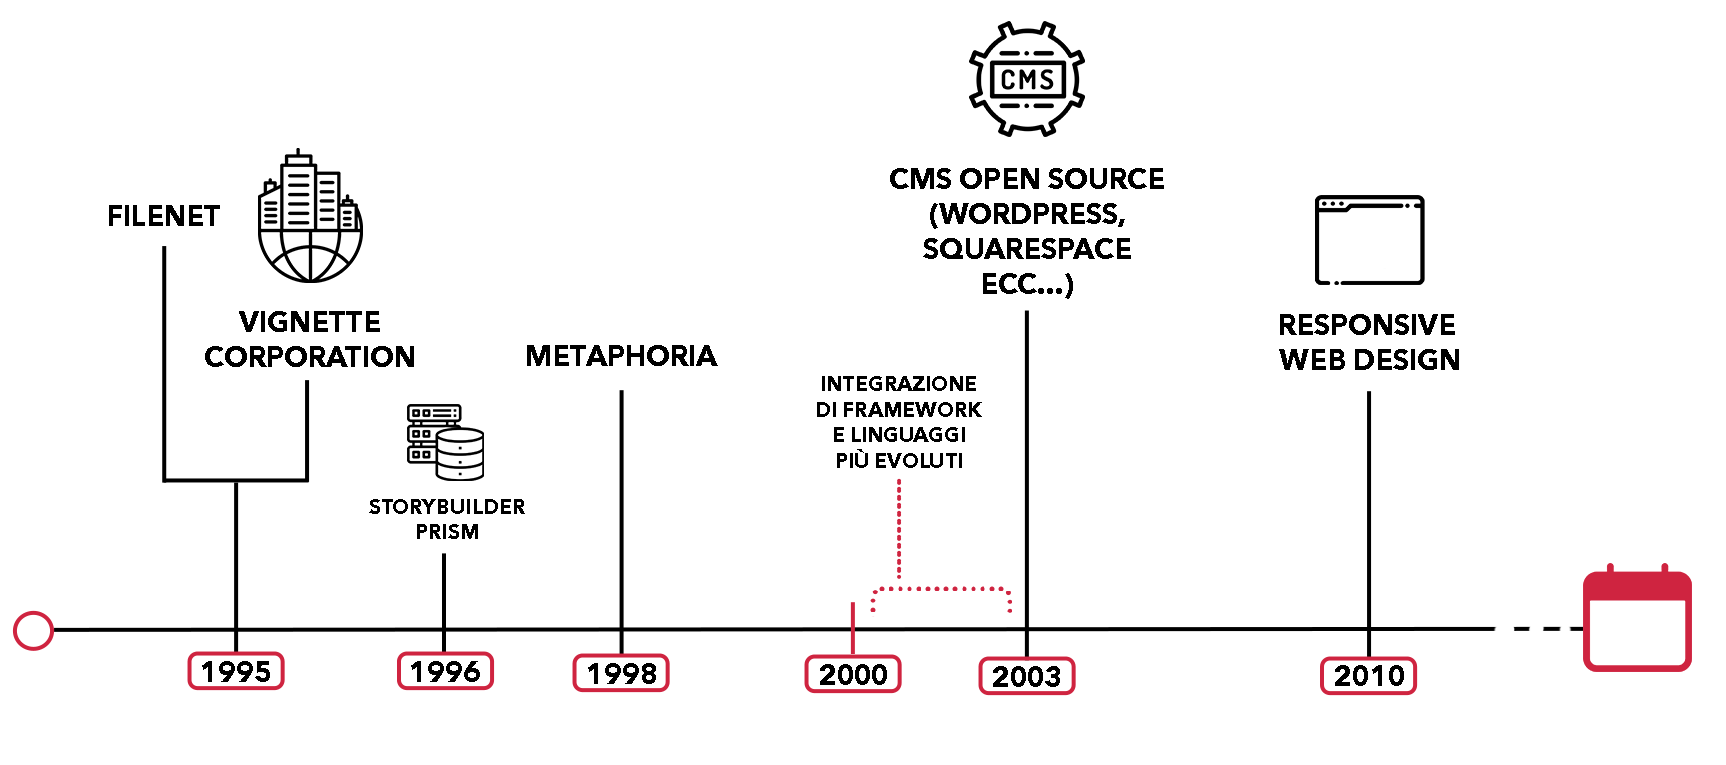
\includegraphics[width=140mm]{images/Storyline.png}
    \caption{Flusso temporale degli eventi\label{overflow}}
\end{figure}


\chapter{Cubo content management system}
\label{chap:CuboCMS}

Il sistema per la gestione dei contenuti Cubo, rientra all'interno della categoria dei CMS proprietari e rappresenta una valida soluzione per lo sviluppo e la realizzazione di un sito web.\hfill \break
Lo strumento è stato sviluppato facendo fede a dei concetti cardine, ovvero flessibilità, modularità, scalabilità, accessibilità in termini d'uso e semplicità per quanto ne riguarda l'interazione da parte del cliente mediante l'utilizzo di strutture ad-hoc per la gestione delle pagine.\hfill \break
Seguirà un'analisi dei linguaggi e degli strumenti utilizzati, susseguita da supervisione globale all'interno della quale verrà analizzato il workflow in merito alla stesura e allo sviluppo del prodotto richiesto dal cliente.
\clearpage
\section{Linguaggi di programmazione}
Il linguaggio di programmazione[1] è un linguaggio formale che specifica un insieme di istruzioni utilizzate per produrre dati in uscita in merito al controllo del comportamento di una macchina formale (tipicamente, un computer) attraverso la stesura in fase di programmazione del codice sorgente, un particolare tipo di testo che definisce il flusso di esecuzione delle operazioni che devono essere eseguite.\hfill \break
Nella produzione di un CMS vengono impiegati linguaggi differenti, scelta dovuta all'eterogeneità che di base si vuole mettere a disposizione dell'utente, come ad esempio la parte grafica a discapito della zona adibito al coordinamento dei contenuti che di per se presenta una struttura logica completamente differente in relazione alla gestione delle risorse, delle strutture dati e dell'utilizzo delle espressioni.
\subsection{Sviluppo back-end}
Il back-end rappresenta la parte del codice che elabora i dati e con la quale l'utente interagisce indirettamente. Di norma, non è presente all'interno di siti web statici (ovvero con contenuti non modificabili).
Dal punto di vista della programmazione ed in riferimento alla sezione d'interesse, la parte di back-end è stata sviluppata mediante l'utilizzo dei seguenti linguaggi:
\begin{itemize}
    \item \textbf{Python}: linguaggio di programmazione ad alto livello multi-paradigma, orientato agli oggetti ed adatto allo sviluppo di applicazioni distribuite. Tra le varie caratteristiche emergono l'utilizzo di variabili non tipizzate, l'indentazione per la sintassi specifica, capacità di overloading e la presenza di un ricco assortimento di tipi, funzioni e librerie standard.
    \item \textbf{JavaScript}: linguaggio di programmazione orientato agli oggetti e agli eventi nato nel 1995 per essere utilizzato nello sviluppo lato client (nel contesto web front-end) ed in seguito esteso anche al lato server. Viene sostanzialmente utilizzato come linguaggio integrato secondo diversi framework che ne consentano l'impiego server-side per la generazione di applicazioni che devono rispondere a numerose richieste in modo rapido ed efficiente.
\end{itemize}
La scelta del voler utilizzare python come linguaggio principale ricade sulla semplicità in termini sintattici, i framework messi a disposizione sono meno frammentati ed incentrati in un impiego ben definito (e.g. Django per lo sviluppo web), sia per la flessibilità e la generalità negli ambienti di utilizzo, che risultano essere molteplici (Web development, Machine Learning ecc...).
\subsection{Sviluppo front-end}
Il front-end è quella parte che si occupa della gestione delle interazione con l'utente per la produzione di dati in ingresso (trattati ed elaborati successivamente in ottica back-end per la produzione in output degli stessi).\hfill \break
Come linguaggio di programmazione, è stato utilizzato \textbf{JavaScript} (discusso nella sezione 3.1.1) per lo sviluppo dello scripting integrato alla realizzazione di applicazioni web dinamiche. \hfill \break
In termini trasversali, sono stati adottati i seguenti linguaggi:
\begin{itemize}
    \item \textbf{HTML}: sviluppato nel 1990, l'Hypertext Markup Language è un linguaggio di markup a dominio pubblico
    rappresentante uno standard per la definizione dei documenti all'interno del World Wide Web.
    \item \textbf{CSS}: pubblicato per la prima volta verso il termine del 1996, il Cascading Style Sheet é un linguaggio utilizzato per la definizione e la formattazione in termini grafici dei documenti scritti in un linguaggio di markup (e.g HTML).
\end{itemize}

\section{Framework e strumenti utilizzati}
Nello sviluppo di un CMS o di un applicativo in generale, con il progredire del tempo, ha preso campo l'utilizzo dei framework, architetture logiche caratterizzate da un insieme di classi astratte correlate tra di esse che in fase d'implementazione, vanno ad inizializzare e a definire un'infrastruttura generale per permettere la semplificazione in merito all'operato del programmatore in fase di progettazione software. Il loro scopo è quello di far risparmiare allo sviluppatore la riscrittura del codice ed evitare il fenomeno della ridondanza favorendo la sinteticità del codice. I vantaggi dell'utilizzo di questo particolare tipo di costrutto sono l'ottimizzazione dei tempi, l'organizzazione del codice e la messa a punto di funzionalità specifiche per determinati tipi di esigenze.
Nella scelta del framework è importante valutare il tipo di applicazione e l'architettura desiderata, evitando di focalizzarsi unicamente sulle caratteristiche tecniche messe a disposizione.\hfill \break
Per il CMS cubo, sono stati adottati i seguenti quadri strutturali:
\begin{itemize}
    \item \textbf{Django}: Web framework open source per lo sviluppo di applicazioni web strutturato secondo il paradigma MVT (Model-View-Template).
    Il progetto venne sviluppato dalla Django Software Foundation e successivamente distribuito nel 2005, mediante licenza BSD (senza copyleft). Tra le varie funzionalità spiccano l'astrazione del database relazionale ad oggetti con supporto multi-piattaforma, un sistema di template basato su tag ereditari ed un sistema per la gestione degli utenti con autenticazione mediante applicazione web.
    \item \textbf{Vue.js}: Framework JavaScript open source per la creazione di interfacce utente e single-page applications. È stato creato da Evan You, ex dipendente Google, che lo ha versionato e distribuito nel 2014. Offre un'ottima adattabilità associata al concetto della scalabilità, fattori chiave nello sviluppo delle applicazioni web.
\end{itemize}

\subsection{API Web}
Per semplificare ulteriormente l'operato del programmatore, sono state utilizzate le API (acronimo di Application Programming Interface)[2], un set di definizioni e protocolli con i quali vengono realizzati e integrati software applicativi. L'obiettivo è quello di semplificare la possibilità di dialogo tra un'applicazione e l'altra garantendo allo stesso tempo amministrazione e flessibilità.
Vengono largamente utilizzate per l'accoppiamento con software di terze parti, favorendo la migrazione verso lo sviluppo di un modello d'architettura orientata ai servizi (SOA, Service Oriented Architecture). \hfill \break
Per l'accesso ai web services, sono state integrate le API RESTful, strutturate secondo i vincoli architettonici REST (acronimo di REpresentional State Transfer).

\begin{figure}[ht!]
    \centering
    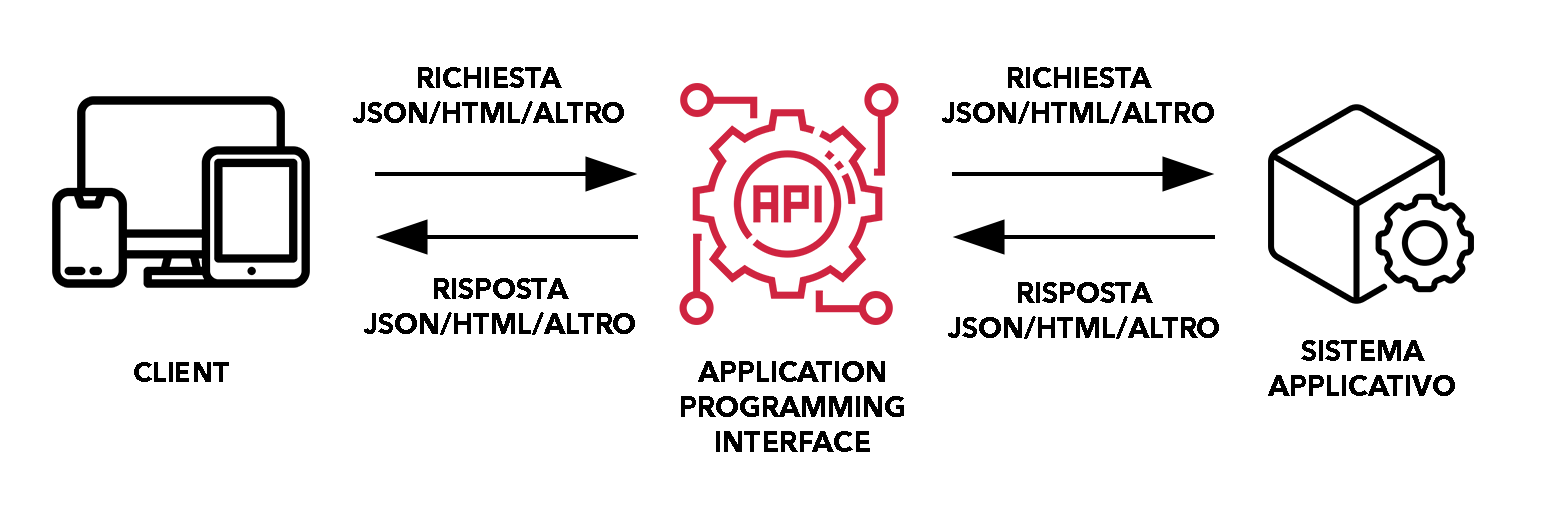
\includegraphics[width=150mm]{images/API.png}
    \caption{Rappresentazione concettuale di un'API\label{overflow}}
\end{figure}

Quando il client inoltra una determinata richiesta, l'API trasferisce al richiedente (o all'endpoint) uno stato rappresentativo della risorsa che, tramite protocollo HTTP, viene consegnata in uno dei diversi formati disponibili (e.g. JSON, HTML, PHP, testo semplice).
\clearpage
Le API sono definibili RESTful se rispettano i seguenti sei vincoli:
\begin{itemize}
    \item Un'architettura client-server composta da client, server e risorse, con richieste gestite tramite HTTP.
    \item Una comunicazione client-server stateless, che quindi non prevede la memorizzazione delle informazioni del client tra le richieste GET: ogni richiesta è distinta e non connessa.
    \item Dati memorizzabili nella cache che ottimizzano le interazioni client-server.
    \item Un'interfaccia uniforme per i componenti, in modo che le informazioni vengano trasferite in una forma standard.
    \item Un sistema su più livelli che organizza ogni tipo di server che si occupa di recuperare le informazioni richieste in gerarchie, invisibile al client.
    \item Codice on demand (facoltativo): la capacità di inviare codice eseguibile dal server al client quando richiesto, estendendo la funzionalità del client.
\end{itemize}

La scelta per quanto ne riguarda l'utilizzo delle API in questione è da associare al REST che mette a disposizione i dati sotto forma di risorsa anziché di servizio ed il fatto che vada ad integrare i verbi HTTP come GET, POST, PUT e DELETE, necessari per comunicare al server cosa fare con i dati identificati dall'URL di una specifica risorsa.
\clearpage

\section{Struttura ed architettura} 
All'interno della seguente sezione viene analizzata la struttura e l'architettura del content management system Cubo. 
Nello specifico, vengono trattati gli elementi base sui quali si erge il sistema proprietario con un particolare riferimento all'applicazione degli strumenti e delle tecnologie citate precedentemente, l'impatto dell'implementazione circa eventuali personalizzazioni richieste dal cliente e il workflow dell'interazione e della gestione dei contenuti.

\begin{figure}[ht!]
    \centering
    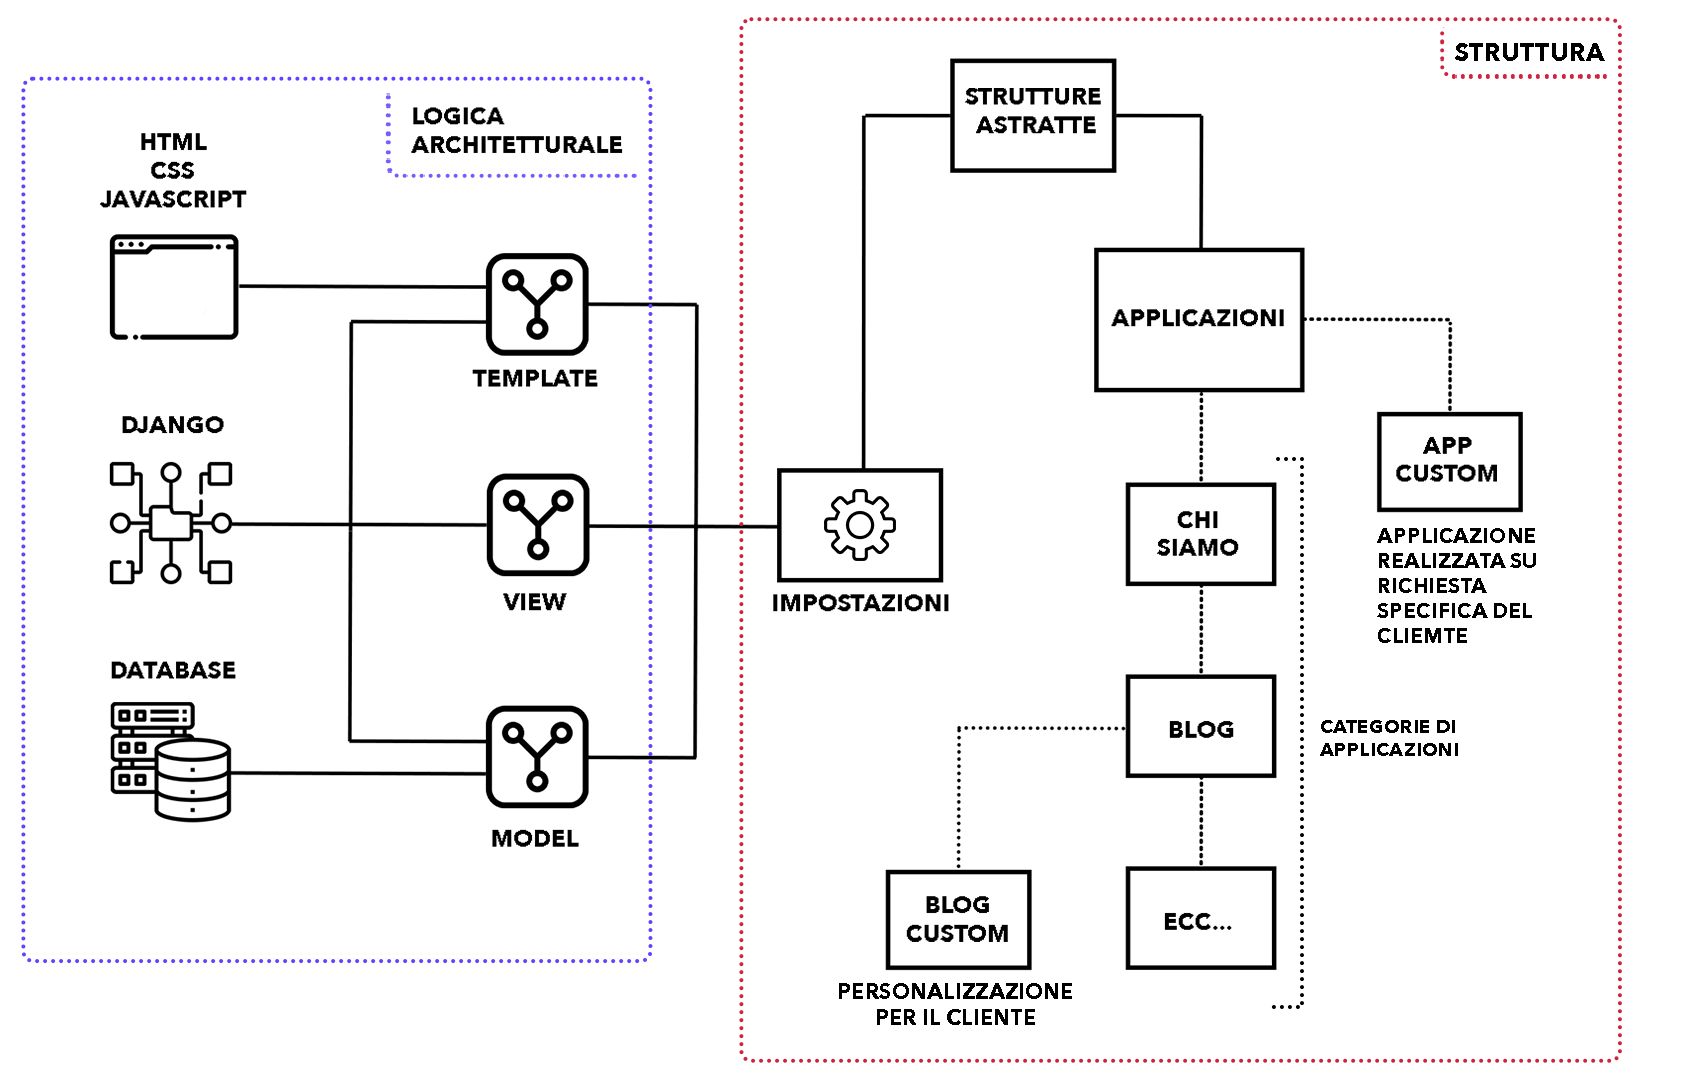
\includegraphics[width=155mm]{images/Cubo CMS Struttura.png}
    \caption{Cubo CMS, struttura ed architettura logica \label{overflow}}
\end{figure}
\clearpage
\subsection{Django e il paradigma MVT}
L'architettura del framework Django (introdotto nel capitolo 3.2) segue i criteri del paradigma Model-View-Template (MVT - Modello, Vista e Template), un pattern utilizzato per lo sviluppo delle applicazioni e delle interfacce Web strutturato secondo i seguenti concetti:
\begin{itemize}
    \item \textbf{Modello}: Un livello astratto dove viene generata e gestita l'infrastruttura per la manipolazione dei dati. All'interno sono presenti delle classi per la rappresentazione delle tabelle contenute all'interno del database e per l'utilizzo delle operazioni CRUD (CREATE, READ, UPDATE, DELETE) in fase d'interazione coi dati.
    \item \textbf{Vista}: Strato incaricato dell'elaborazione delle richieste effettuate da parte degli utenti. Le funzioni che lo stesso mette a disposizione, vengono utilizzate per amministrare le interazioni, estrarre i dati dal database, elaborarli e fornire una risposta rappresentativa attraverso il template.
    \item \textbf{Template}: identificabile attraverso un file utilizzato per la rappresentazione dei dati processati all'interno della vista di riferimento. Presenta una sintassi semplice ed al suo interno avviene la conversione delle informazioni in elementi associabili al linguaggio HTML.
\end{itemize}

\clearpage
\begin{figure}[ht!]
    \centering
    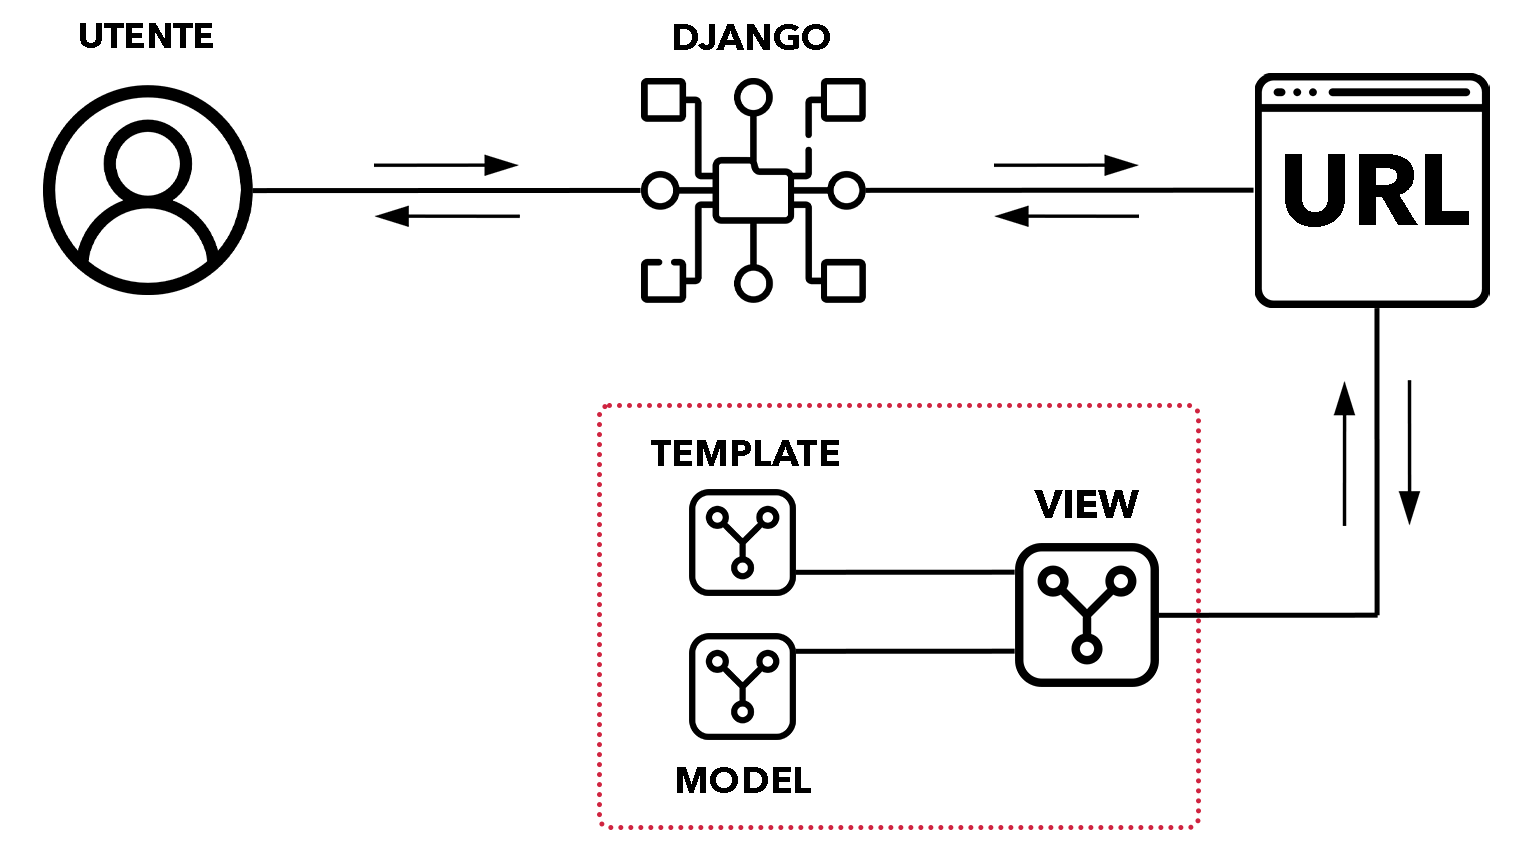
\includegraphics[width=120mm]{images/Paradigma MVT.png}
    \caption{Workflow del paradigma MVT \label{overflow}}
\end{figure}

L'utente effettua una richiesta che viene automaticamente gestita dal framework. Quest'ultimo analizza la disponibilità delle risorse tramite l'URL (Uniform Resource Locator)[3], una sequenza di caratteri che identifica univocamente l'indirizzo di una risorsa. In caso la mappatura dovesse dare esito positivo, si procede con l'utilizzo della funzione per il richiamo della vista che andrà ad interagire con il modello ed il template di riferimento. Una volta generato, il template viene incapsulato all'interno di una risposta presa in carico da Django inviata successivamente all'utente, libero di poterne interagire.

\clearpage

\subsection{Configurazione delle impostazioni}
Le impostazioni sono alla base della predisposizione per quanto ne riguarda l'utilizzo di tutti gli elementi d'interesse presenti all'interno del progetto. \hfill \break
In termini caratteristici, al loro interno troviamo:
\begin{itemize}
    \item \textbf{Ambienti Diversificati}: Ogni ambiente presenta impostazioni e configurazioni specifiche per il coordinamento dei servizi e/o delle strutture.
    \item \textbf{Dati sensibili}: Password del Database, token per API di terze parti, credenziali per l'accesso a determinati servizi.
\end{itemize}

È necessario far uso di una pratica che permetta l'eliminazione dell'errore umano in fase di pianificazione (uno sviluppatore potrebbe andare ad integrare un API e non riuscire ad aggiungere delle impostazioni specifiche per l'utilizzo della stessa all'interno del progetto, andandone a compromettere l'operato su larga scala). 
Dal punto di vista pratico, è stato utilizzato un approccio procedurale: in un primo momento si vanno a definire le applicazioni da implementare all'interno del sito in fase di sviluppo susseguiti dalla definizione delle lingue supportate (su specifica richiesta del cliente), i vari percorsi per poter accedere ai template, ai contenuti grafici e a quelli statici. 
In seguito, si passa agli strumenti per il debug e l'associazione con il database d'interesse (che deve essere già stato inizializzato a priori). 
Si procede con l'instaurazione della Sitemap, un particolare tipo di file contente tutti gli URL presenti all'interno del sito. Il suo obiettivo è agevolare la navigazione client-side migliorando l'impatto nel contesto della scansione e dell'indicizzazione web.
Infine, si va ad ultimare il tutto attraverso la configurazione della WSGI (Web Server Gateway Interface)[4], un protocollo di trasmissione che stabilisce e descrive comunicazioni ed interazioni tra server ed applicazioni web scritte nel linguaggio Python. Il protocollo specifica come i server si facciano carico delle richieste provenienti dai browser/client ed inoltrino le informazioni richieste alle relative applicazioni.


\subsection{Applicazioni}
Il CMS Cubo mette a disposizione diverse applicazioni strutturate secondo l'architettura client-server e focalizzate nell'offrire determinati servizi all'utente client in fase d'interazione sulla base logica del paradigma MVT (discusso precedentemente).\hfill \break
Ogni singola applicazione si articola di tutti gli elementi necessari per un corretto funzionamento, ovvero modelli, viste, template ed URL specifici. \hfill \break
Lo sviluppo avviene mediante l'utilizzo dei modelli astratti, fondamentali in ottica di risparmio e minimizzazione del codice.
All'interno del progetto è presente una particolare applicazione, denominata \textit{Core}, nella quale presenzia tutta la componentistica necessaria per poter mettere in pratica l'approccio nella sua concezione astratta.
Nell'ipotetico esempio della generazione di un \textit{modello} per una determinata applicazione, si procederà con l'importazione del modello astratto \textit{StandardPageMetaModel} (specifico per i modelli) e l'inizializzazione della classe con i relativi \textit{meta-dati} (rappresentati un'insieme di informazioni necessari per una corretta gestione e conservazione nel tempo delle risorse). \hfill \break
\lstinputlisting[firstline=1, lastline=9, caption={Principio dell'eredità applicato al modello}]{code/ExampleModel MVT.py}
Il workflow appena analizzato, utilizza il principio dell'ereditarietà e viene iterato anche nel processo per la generazione delle viste e dei template.\hfill\break
Nel caso dei template si fa utilizzo del file \textit{\_base.html}, che definisce la struttura sulla quale proseguiranno le operazioni di sviluppo front-end. \hfill \break
In ottica architetturale il template fa uso dello sviluppo a blocchi per poter far fede al concetto dell'ottimizzazione e della pulizia del codice. \hfill \break
I blocchi sono delimitati da dei tag che ne definiscono la struttura logico-gerarchica e durante la generazione del template di un'ipotetica applicazione, a seguito dell'importazione del file  \textit{\_base.html} al suo interno, prenderà campo la sovrascrittura dei blocchi di riferimento con successiva implementazione del codice HTML. \hfill \break
\lstinputlisting[firstline=1, lastline=13, caption={Struttura dei blocchi all'interno del \_base.html}]{code/_base.html}
\clearpage
L'ipotetico template dell'applicazione avrà di conseguenza ereditato l'aspetto e la logica sintattica del \textit{Core} template, pronto per essere personalizzato nel caso di una particolare richiesta da parte del cliente.
\lstinputlisting[firstline=1, lastline=5, caption={Sovrascrittura all'interno del template ereditario}]{code/_son.html}

\subsubsection{Modelli astratti}
In fase di programmazione, la gestione e l'ordine del codice sono fondamentali. L'utilizzo dei modelli astratti favorisce una pratica precisa, pulita ed ottimizzata per lo sviluppo del CMS.\hfill \break
Tali modelli, fanno uso del concetto della metamodellazione[5], strutturato sull'analisi, sulla costruzione e sullo sviluppo di strutture, regole, vincoli, modelli e teorie applicabili ed utilizzabili per la modellazione di classi predefinite di problemi.
Mentre il modello rappresenta un'astrazione dell'idea di una determinata entità, il meta-modello si identifica in un ulteriore astrazione dello stesso e con una definizione più approfondita delle strutture e dei vari elementi al suo interno. \hfill \break
Il modello \textit{StandardPageMetaModel} rappresenta un caso concreto della messa in pratica di questo tipologia d'approccio.
Per unificare la metodologia, sono state sviluppate anche innumerevoli classi astratte secondo l'immagine dell'ereditarietà multipla[6], in cui una classe può ereditare funzionalità e caratteristiche da più di una classe base. \hfill \break
All'interno delle viste adibite al servizio amministrativo troviamo classi come \textit{BaseCreate} e \textit{BaseUpdate}, incaricate della gestione form-view, che una volta concretizzate (nel contesto dello sviluppo di un'applicazione), estendono tutte le funzionalità a loro disposizione con una successiva sovrascrittura degli attributi (specifici) d'interesse per la classe appena inizializzata.


\subsection{Database}
Il database è un sistema informatico attuo alla memorizzazione permanente dei dati ed in senso tecnico, può essere definito com un archivio strutturato per la conservazione e il mantenimento dei dati. Il framework Django, utilizza i modelli per interagire con database e sempre secondo il concetto della programmazione orientata agli oggetti. \hfill \break
Il modello, pertanto, si identifica nella forma di un oggetto caratterizzato da determinate proprietà. All'interno del database, quest'ultimo assume l'aspetto di una tabella, a sua volta popolata da righe e colonne, che ne rappresentano rispettivamente le istanze e gli attributi. In seguito, tra le varie tabelle, vengono definiti i vincoli e le associazioni alla base della logica relazionale adottata.
Il modelli e le tabelle costituiscono un dualismo che deve procedere in maniera sincrona per poter garantire un mantenimento efficiente delle risorse e dell'infrastruttura adibita all'interrogazioni del database.
Django utilizza le migrazioni per prorogare ed apportare eventuali modifiche effettuate sui modelli al database con una diretta e conseguente generazione del file di migrazione, un particolare tipo di documento all'interno del quale viene tenuta traccia di tutte le variazioni effettuate dalla suddetta procedura.

\clearpage

\subsection{Console di amministrazione}
Dopo aver ultimato tutte le strutture ed aver configurato in maniera specifica tutte le varie impostazioni, il sito si prepara ad essere popolato secondo i parametri e i contenuti d'interesse. Cubo CMS predispone un pratico pannello di amministrazione all'interno del quale è possibile andare ad inserire, gestire e supervisionare tutti gli elementi che si reputano opportuni. La dashboard è stata strutturata in maniera da predisporre un utilizzo facile ed intuitivo per l'utente amministratore. Ogni applicazione, all'interno del pannello, presenta una sezione dedicata dove è possibile andarne a modificare ogni aspetto correlato al contesto amministrativo della stessa in maniera indipendente nel rispetto delle altre applicazioni installate.

\begin{figure}[ht!]
    \centering
    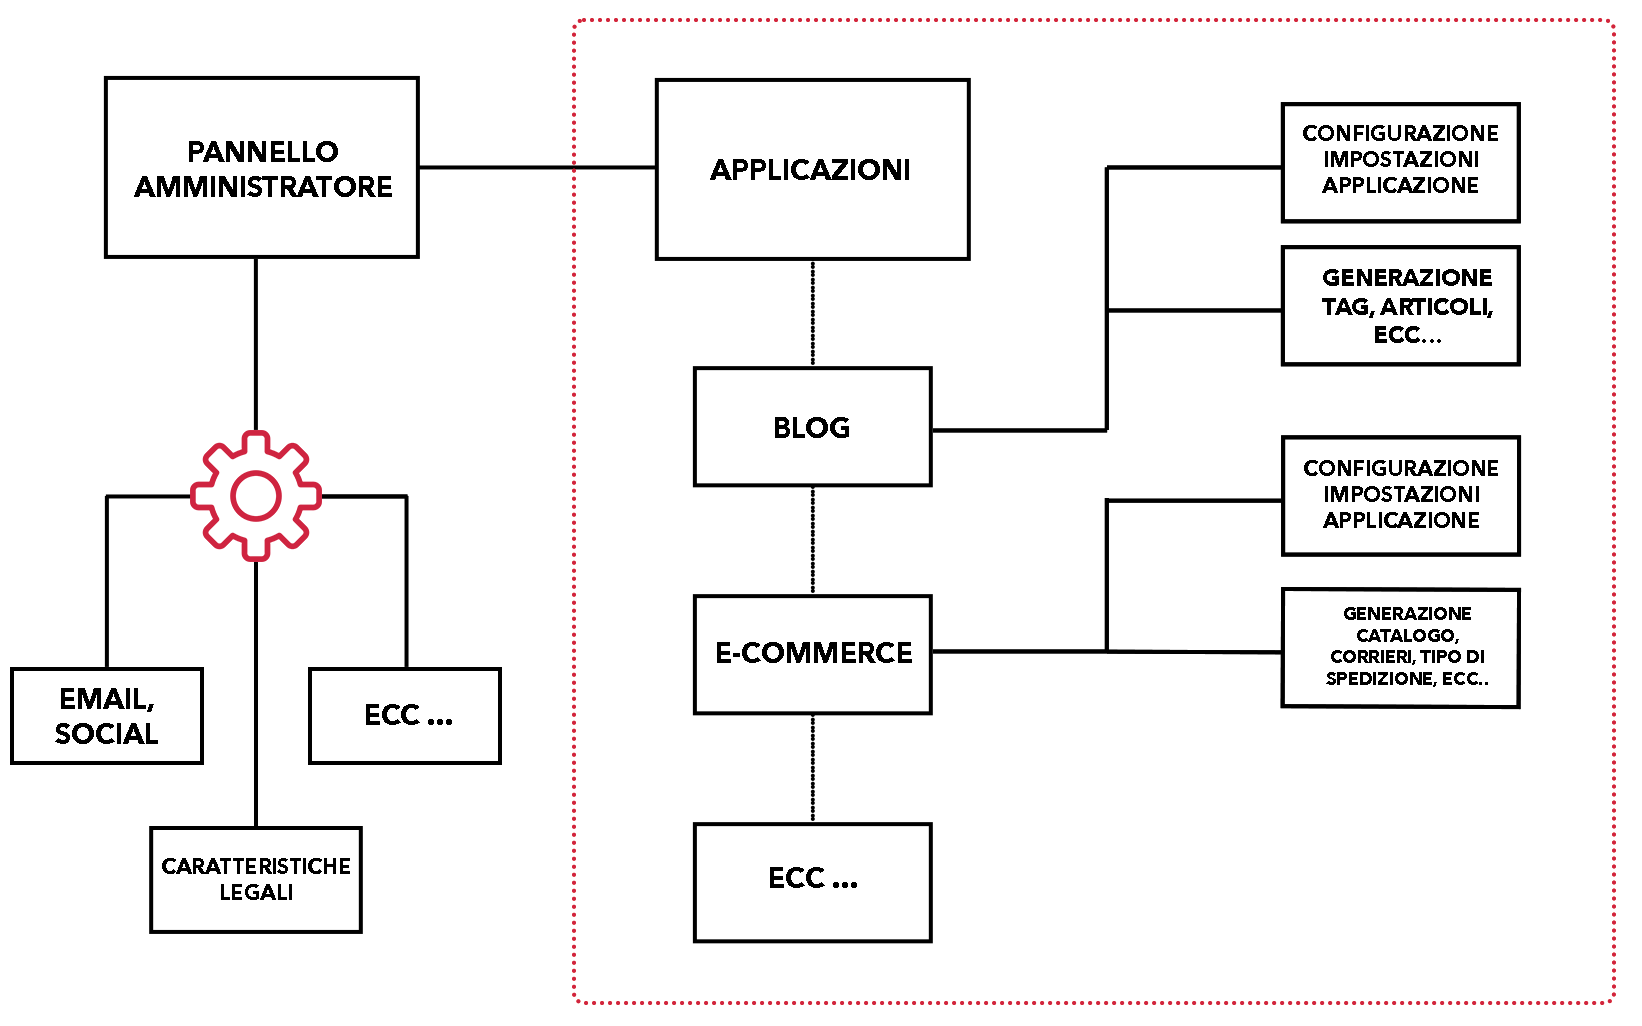
\includegraphics[width=140mm]{images/Struttura Console amministrazione.png}
    \caption{Struttura della console amministrativa\label{overflow}}
\end{figure}

\subsubsection{Blocchi per la personalizzazione}
Il sistema per la gestione dei contenuti deve adattarsi alle richieste e alle esigenze del cliente. A tal proposito, la personalizzazione del sito riveste un ruolo fondamentale e lo strumento mette a disposizione diverse funzionalità per poter procedere in questa direzione. In termini tecnici, come molti altri CMS, anche Cubo fornisce dei blocchi, ovvero dei moduli preconfigurati che possono essere utilizzati per la costruzione del sito nelle sue componentistiche (come ad esempio per le testate, i footer, le sezioni dedicate ad un determinato contenuto, la modifica del logo del sito ecc...).\hfill \break
L'utilizzo dei blocchi estende il concetto della modularità e della flessibilità. Attraverso i seguenti costrutti, l'amministratore può modificare a suo piacimento l'estetica e i contenuti presenti all'interno delle differenti pagine, senza la necessità di particolari conoscenze tecniche. Allo stesso tempo, l'implementazione di questo tipo di approccio ha uniformato ulteriormente le pratiche in fase di programmazione, evitando costanti modifiche sulla base della particolari commesse da parte del cliente.

\chapter{Progettazione e deployment su infrastruttura Cloud}
\label{chap:ProgettazioneCloud}
Il CMS mette a disposizione una struttura articolata attraverso la quale è possibile realizzare molteplici siti web secondo specifiche richieste.
Altrettanto importante e l'erogazione, la gestione e il mantenimento del servizio, che dovrà risultare accessibile attraverso l'utilizzo di un determinato dominio web, ovvero un indirizzo univoco utilizzato per richiamare un sito internet associato. \hfill \break
Nella scelta e nella messa in pratica di degli strumenti necessari per lo sviluppo in cloud, risulta fondamentale soddisfare determinati criteri e garantire velocità, scalabilità, produttività, prestazioni degne di nota susseguite dall'affidabilità e dalla sicurezza.
All'interno di questo capitolo seguirà l'analisi e il confronto tra le varie tipologie di infrastrutture disponibili, l'approccio utilizzato per la gestione dei dati e la metodologia utilizzata per l'interazione con gli stessi per poter poi procedere con lo studio dei mezzi utilizzati per la distribuzione dei diversi elementi d'interesse e concludendo il tutto con un approfondimento circa le scelte effettuate e le corrispettive motivazioni.

\section{Scelta dell'infrastruttura}
Nella gestione degli ambienti e dei servizi, la scelta dell'infrastruttura[7] è significativa. Con tale termine, si va ad intendere la combinazione di più apparati e sottosistemi interconnessi tra di loro secondo un'architettura di tipo client-server, preposti per mettere a disposizione funzionalità e servizi a favore degli utenti. I principali obiettivi sono:
\begin{itemize}
    \item Offrire un storage ad alte prestazioni dei dati.
    \item Mettere a disposizione una rete a bassa latenza per ridurre il ritardo nel flusso dei dati e agevolare le comunicazioni tra i vari elementi architetturali.
    \item Garantire sicurezza e affidabilità mediante controlli all'accesso delle informazioni.
    \item Mettere a disposizione la virtualizzazione per poter fornire server più veloci ed un conseguente aumento del tempo di attività.
    \item Ridurre le interruzione e garantire continuità del servizio.
\end{itemize}

Le infrastrutture presentano proprietà ed elementi articolati, che possono essere suddivisi in due grandi categorie, l'hardware e il software.
Queste due classi, rappresentano un binomio altamente consolidato e sono vincolate da un utilizzo reciproco in quanto inutilizzabili in maniera singolare.
Con il termine hardware, si fa riferimento ai server, data center, hub e strutture fisiche di vario genere impiegate nel mantenimento effettivo dei dati.
Il software rappresenta l'insieme dell'istruzioni logico-digitali presenti all'interno del sistema con i quali non è possibile interagire.
Ad oggi, il mercato mette a disposizione diverse soluzioni per quanto ne riguarda il tipo d'infrastruttura adottabile secondo concezioni ed applicazioni divergenti.

\subsection{Impianto tradizionale}
L'infrastruttura tradizionale mette a disposizione un eco-sistema dedicato interamente gestito dall'azienda. Architetturalmente parlando, sono presenti strutture (come server, data center e hardware di rete) di riferimento per il mantenimento, la gestione dei dati e la componentistica per lo sviluppo in rete (switch, router e hub).
Questa soluzione garantisce un'estrema flessibilità nell'utilizzo e nell'impiego delle periferiche, affidabilità, scalabilità e svincola l'azienda dal doversi interfacciare con enti di terza parte per l'utilizzo di servizi esterni.
In contrapposizione, è necessaria la presenza del personale qualificato che garantisca:
\begin{itemize}
    \item Implementazione adeguata dell'infrastruttura
    \item Corretta gestione del database
    \item Svolgimento a cadenza regolare del backup dei dati
    \item Manutenzione in caso di guasti e/o malfunzionamenti
    \item Sistema per la gestione dell'architettura sempre in costante aggiornamento
    \item Amministrazione in merito alla sicurezza e l'accesso alla rete
\end{itemize}
Il principale svantaggio è correlabile ai costi per il mantenimento, sia dal punto di vista del materiale che dei sistemisti incaricati dei vari compiti precedentemente citati.

\subsection{Cloud computing}
L'infrastruttura cloud sfrutta il paradigma del cloud computing[8] per l'erogazione di servizi offerti su richiesta da un fornitore a un cliente finale attraverso la rete internet (come l'archiviazione, l'elaborazione o la trasmissione dati), a partire da un insieme di risorse preesistenti, configurabili e disponibili in remoto sotto forma di architettura distribuita. Si basa sul concetto della virtualizzazione, la componentistica non è di proprietà della azienda ma viene erogata sotto forma servizio dal fornitore qualificato. Attraverso un'interfaccia ad-hoc, il cliente amministratore può selezionare un determinato servizio e configuralo secondo le esigenze del cliente finale che ha commissionato il lavoro iniziale, seguendo un approccio transitivo.
Il paradigma mette a disposizione due particolare modelli per il contesto di riferimento:
\begin{itemize}
    \item \textbf{Modello IaaS} \textit{(Infrastructure as a Service)}: garantisce al cliente l’accesso ad un'infrastruttura con a disposizione tutti gli elementi necessari per poter proseguire con le operazioni di sviluppo. Il servizio garantisce un'alta scalabilità e si predispone secondo il concetto del pay-per-use, in modo che il cliente paghi solo per quanto stia realmente utilizzando. Tra i vantaggi presenzia il fatto dell'assenza sui costi dell'hardware e per quanto ne riguarda la configurazione, la modernizzazione e l'eventuale manutenzione, la possibilità di inizializzare nuovi progetti e averli a disposizione in tempi brevi ed infine l'alta scalabilità per l'accesso e la gestione delle risorse. I principali svantaggi sono il vincolo operazionale al quale ci si lega con il provider in termini di disponibilità delle strutture, sicurezza e protezione dei dati e nell'eventuale migrazione verso un altro fornitore.
    \clearpage
    \item \textbf{Modello PaaS} \textit{(Platform as a Service)}: mette a disposizione l'ambiente e gli strumenti necessari per poter sviluppare ed operare in cloud. Questa scelta, solleva l'azienda dal doversi occupare delle gestione dell'infrastruttura, interamente amministrata dal provider. La suddetta soluzione, garantisce uno sviluppo più facile e veloce, prestazioni scalabili ed adattabili al contesto nel quale il servizio è applicato ed una netta riduzione dei costi (dovuta al risparmio dell'hardware ma anche del software, come il sistema operativo, l'ambiente di sviluppo e linguaggio di programmazione, messi a disposizione dal fornitore). L'elemento negativo è rappresentato dal fatto che il cliente non abbia nessun tipo di controllo sull'infrastruttura.
\end{itemize}

\begin{figure}[h]
    \centering
    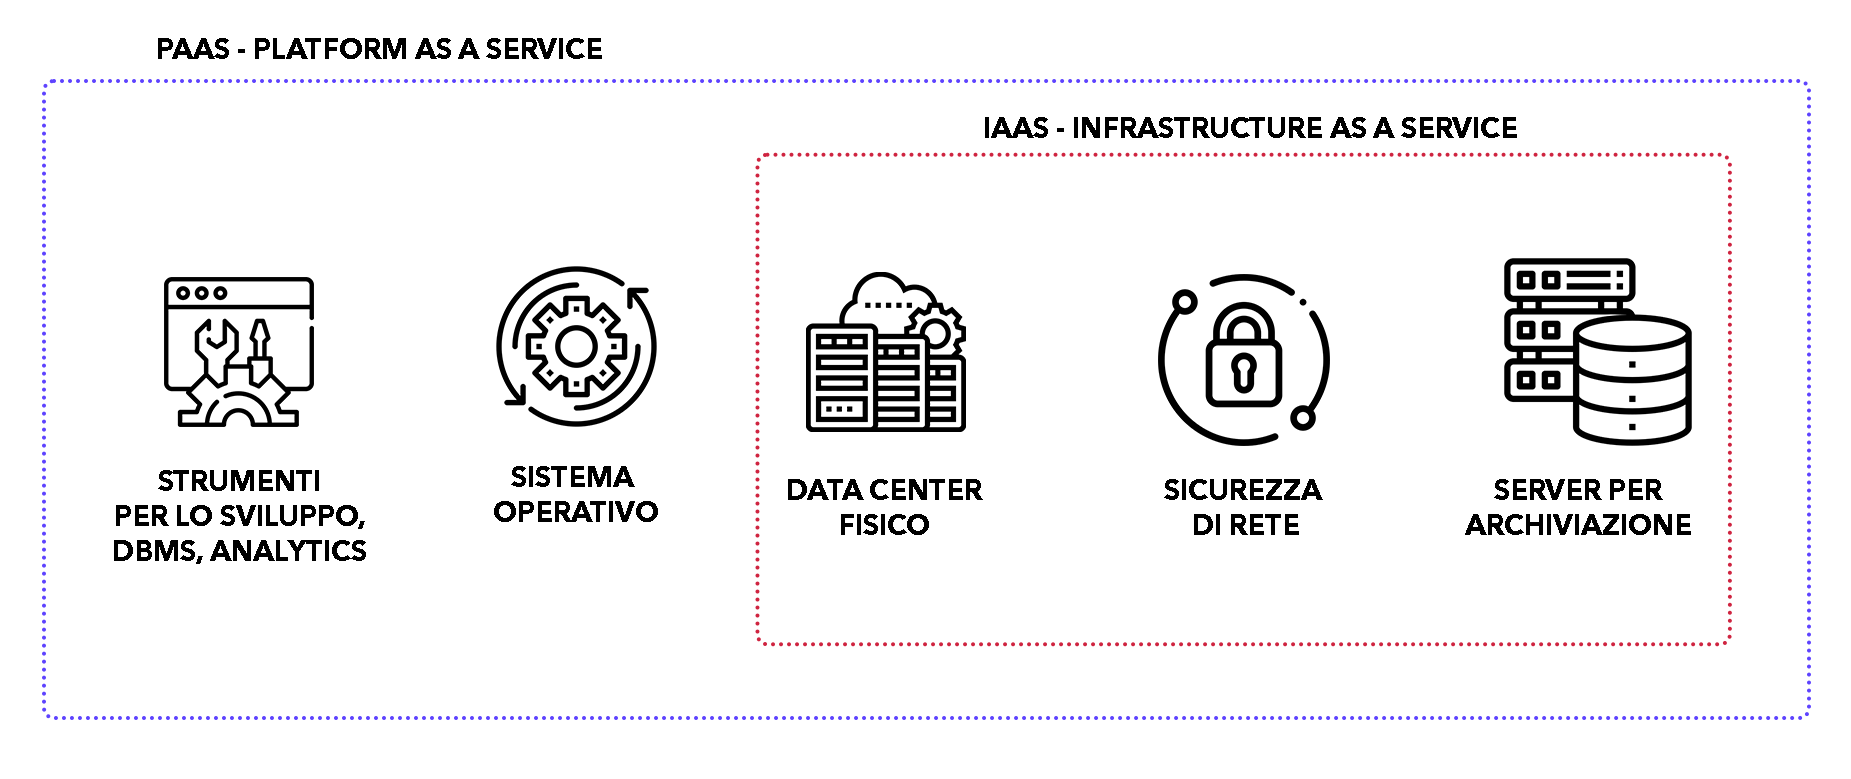
\includegraphics[width=150mm]{images/Infrastrutture.png}
    \caption{Modelli Cloud \label{overflow}}
\end{figure}

\clearpage

\section{L'importanza della CDN}
La rete per la distribuzione dei contenuti (CDN - Content Delivery Network) è un sistema di server interconnessi che collaborano in maniera convergente per l'erogazione di diversi servizi in direzione degli utenti finali. Il CDN si avvale dell'utilizzo del caching, un particolare tipo di processo che si occupa di memorizzare, in maniera temporanea, una copia del file d'interesse per permettere un accesso molto più rapido allo stesso, tramite un server posizionato nelle vicinanze dell'utente prossimo ad accedere alla risorsa. Dal punto di vista topologico, i data center presentano una architettura distribuita in aree geografiche differenti. Tale strumento  permette un accesso molto più rapido ai contenuti messi a disposizione da una determinata struttura. \hfill \break
In termini pratici, è possibile ipotizzare che un utente si trovi in America e che nel frattempo stia cercando di accedere ad un sito europeo. Il caricamento degli elementi risulterà piuttosto lento. La CDN va a predisporre una copia dei contenuti all'interno di un server allocato in America, permettendo al client un accesso molto più rapido al sito in questione e ai relativi servizi messi a disposizione. \hfill \break
Le CDN, con il passare del tempo, sono diventate indispensabili. I principali motivi per quale risulta necessario farne uso sono:
\begin{itemize}
    \item Garanzia di esperienze rapide, affidabili e coerenti con il target prestazionale attraverso il quale si cerca di fornire un determinato tipo di servizio.
    \item Riequilibrio e gestione del traffico dati, per poter offrire contenuti nel miglior modo possibile.
    \item Maggiore sicurezza da parte degli utenti.
    \item Ottimizzazione dell'indicizzazione in merito alle diverse località geografiche.
\end{itemize}
Tra gli svantaggi emergono i costi per l'utilizzo di una CDN di qualità e le procedure di attivazione in riferimento alla configurazione manuale dei percorsi all'interno del sito, l'upload dei diversi contenuti statici e le modifiche per l'integrazione all'interno del CMS.


\section{DataBase Management System}
Il database si occupa del mantenimento delle risorse ed è necessario adottare specifici strumenti per poter interagirci nel migliore dei modi.
Il DataBase Management System rappresenta la soluzione attrverso la quale è possibile interfacciarsi con l'archivio dati. Tramite il DBMS[9], è possibile creare, manipolare ed interrogare un efficiente database ospitato su architettura hardware dedicata oppure su un semplice computer.
La struttura è stata progettata secondo il concetto multi-utente a sua volta basato su una gestione multitasking delle varie operazioni eseguibili al di sopra di un'infrastruttura di rete abilitata per l'accesso alla base di dati.

\begin{figure}[ht!]
    \centering
    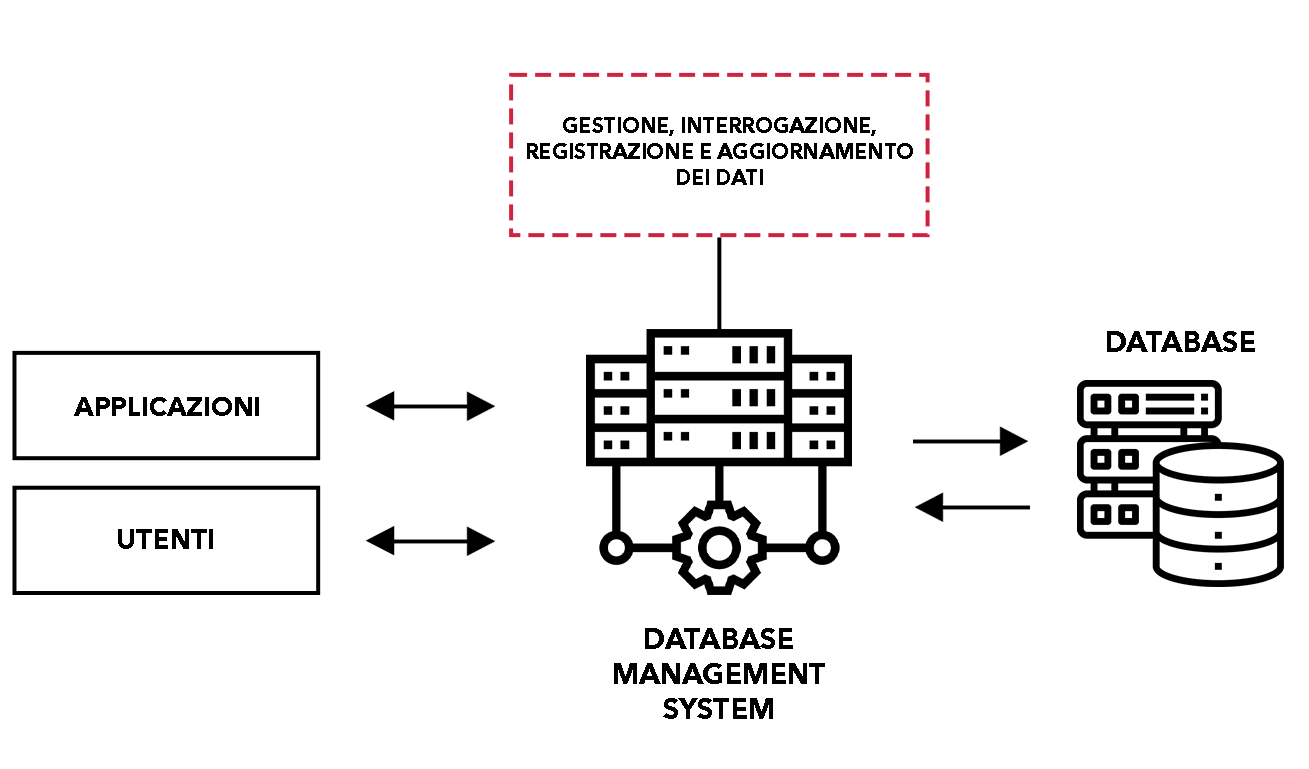
\includegraphics[width=140mm]{images/DBMS.png}
    \caption{Database Management System (DBMS)\label{overflow}}
\end{figure}

\clearpage

\subsection{Caratteristiche, differenze e vantaggi}
Per la strutturazione dei dati, il DBMS implementa al suo interno un modello logico rappresentativo. Ad oggi il settore offre molteplici soluzioni, che possono essere catalogate all'interno di due grandi famiglie:
\begin{itemize}
    \item \textbf{Structured Query Language (SQL)}: Utilizzano un linguaggio specifico per poter effettuare operazioni di manipolazione dei dati all'interno di un database strutturato secondo il modello relazionale, ovvero costituito da tabelle bidimensionali articolate in righe (tuple) e colonne (attributi). In questa tipologia, si fa forza il concetto dell'astrazione secondo il quale l'interazione avviene nel rispetto della rappresentazione logica delle risorse (e non fisica).
    \item \textbf{Not Only Structured Query Language (NoSQL)}: Presentano una schematizzazione flessibile e realizzata ad-hoc per il soddisfacimento di un determinato caso d'uso. A differenze del linguaggio SQL, i dati vengono memorizzati in un formato predefinito (solitamente JSON) e sono ottimizzati per uno sviluppo semplice e per una scalabilità orizzontale.
\end{itemize}
Il DBMS assicura semplicità nell'accesso alla struttura e al tempo stesso garantisce consistenza, privatezza e affidabilità. I principali vantaggi sono:
\begin{itemize}
    \item \textbf{Linguaggio d'interrogazione universale}: Ogni DBMS predispone l'utilizzo di un determinato linguaggio (SQL nel modello relazionale) che permetta la creazione delle strutture per il contenimento dei dati, l'inserimento, la cancellazione e l'aggiornamento degli stessi.
    \item \textbf{Indipendenza dei dati}: Grazie all'astrazione dei dati, il DBMS si avvale della creazione di specifici file (indici) per poter accedere al database che di norma è memorizzato su un disco secondario ottimizzando il tutto nell'ottica della velocità e dell'efficienza.
    \item \textbf{Controllo della ridondanza}: il software analizza la presenza di eventuali dati logici duplicati e predispone gli strumenti per poter gestire tale eventualità (il suddetto fenomeno potrebbe generare inconsistenza oltre ad un inevitabile maggior utilizzo della memoria).
    \item \textbf{Vincoli d'integrità}: è permesso specificare eventuali vincoli al fine di garantire l'integrità e l'omogeneità concettuale dei dati.
    \item \textbf{Operazioni atomiche}: Il sistema permette l'effettuarsi di una sequenza di operazioni che deve avvenire con successo, in caso contrario ogni singola operazione viene annullata e la base di dati non subisce alterazioni.
    \item \textbf{Accesso concorrente}: é possibile accedere in maniera contemporanea al database senza incorrere ad eventuali anomalie.
    \item \textbf{Privatezza ed affidabilità}: il sistema garantisce un accesso protetto ai dati per conto di utenti specifici e fornisce metodi per il salvataggio o il ripristino del database in caso di guasti e/o anomalie.
\end{itemize}

\clearpage

\section{Implementazioni effettuate}
Dopo aver analizzato tutti gli elementi d'interesse per l'erogazione dei servizi, vengono elencate e motivate tutte le scelte effettuate in merito alla distribuzione e l'implementazione delle varie infrastrutture. \hfill \break
Per il deployment è stato scelto un approccio in Cloud di tipo PaaS (Platform as a Service). La decisione è stata quella di adottare il servizio di \textbf{Heroku} per la distribuzione e la gestione degli applicativi. La struttura garantisce un alta scalabilità, il supporto multi-linguaggio nell'ambito della programmazione e mette a disposizione una Git (un software per il controllo distribuito della versione utilizzabile tramite interfaccia a linea di comando) per la gestione delle modifiche sulla repository del progetto.\hfill \break
Come rete per la distribuzione dei contenuti, la scelta è ricaduta sull'utilizzo del CDN \textbf{Cloudflare}. Il servizio garantisce il processo di caching, un ottimo filtraggio del traffico in entrata, un efficiente sistema DNS (Domain Name System) per la risoluzione dei domini nei corrispettivi indirizzi IP (e viceversa), sicurezza e protezione contro il traffico malevolo. \hfill \break
Infine, per quanto ne riguarda la scelta del DBMS, è stato implementato \textbf{PostgreSQL}, strutturato secondo un modello logico-rappresentativo ad oggetti che garantisce una maggiore coerenza tra il database ed il linguaggio programmazione oltre che all'instaurazione di query ad elevate complessità per l'interrogazione dell'archivio.
\chapter{Conclusioni e Sviluppi Futuri}
\label{chap:Conclusioni}

Il World Wide Web è un mondo in costante evoluzione è lo sviluppo degli strumenti deve procedere a pari passo con esso. All'interno del documento sono stati presi in considerazione tutti gli aspetti del CMS a partire dai linguaggi utilizzati fino all'infrastruttura per la distribuzione del servizio. L'approccio messo in pratica in fase di sviluppo ha dato alla nascita un sistema flessibile e scalabile in grado di adattarsi a molteplici situazioni senza andare a sfigurarne la struttura sulla quale si erge il tutto. Lo strumento ha subito un processo di convalida attraverso il quale è stata garantita la conformità all'uso e alle esigenze dell'utente secondo gli aspetti della sicurezza e della gestione dei contenuti.
Le aspettative in fase di progettazione sono state rispettate e le applicazioni web sono tutt'ora in esecuzione all'interno del contesto online. Cubo offre una soluzione professionale per la realizzazione dei siti web e in futuro l'azienda ha pianificato un rilascio open source dello strumento come una valida alternativa ai competitors attualmente disponibili sul mercato.


%%%%%%%%%%%%%%%%%%%%%%%%%%%%%%%%%%%%%%%%%%%%%%%%%%%%%%%%%%%%%%%


% BIBLIOGRAFIA
\begin{thebibliography}{9}
\bibitem{}
        Wikipedia.org,
        \textit{Linguaggi di programmazione}.
        \hfill\break
    \bibitem{}
        Redhat.com,
        \textit{What are Application Programming language}
        \hfill\break
    \bibitem{}
        Wikipedia.org,
        \textit{Uniform Resource Locator}.
        \hfill\break
    \bibitem{}
        Wikipedia.org,
        \textit{Web Server Gateway Interface}.
        \hfill\break
    \bibitem{}
        Wikipedia.org,
        \textit{Metamodellazione}.
        \hfill\break
    \bibitem{}
        Html.it,
        \textit{L'ereditarietà multipla}.
        \hfill\break
    \bibitem{}
        Wikipedia.org,
        \textit{Sistema Informatico}.
        \hfill\break
    \bibitem{}
        Wikipedia.org,
        \textit{Cloud Computing}.
        \hfill\break
    \bibitem{}
        Wikipedia.org,
        \textit{Database Management System}.

\end{thebibliography}

\end{document}
